\documentclass[aspectratio=169,11pt]{beamer}
\usepackage[T1]{fontenc}
\usepackage{lmodern}
\usepackage{booktabs,tabularx,amsmath,graphicx}
\definecolor{Navy}{HTML}{102C43}
\definecolor{Teal}{HTML}{007F82}
\definecolor{Ink}{HTML}{243746}
\definecolor{Muted}{HTML}{637482}
\setbeamercolor{normal text}{fg=Ink,bg=white}
\setbeamercolor{structure}{fg=Teal}
\setbeamercolor{frametitle}{fg=Navy}
\setbeamercolor{title}{fg=Navy}
\setbeamercolor{subtitle}{fg=Teal}
\setbeamercolor{footline}{fg=Muted}
\setbeamerfont{title}{size=\LARGE,series=\bfseries}
\setbeamerfont{frametitle}{size=\Large,series=\bfseries}
\setbeamerfont{subtitle}{size=\large}
\setbeamertemplate{navigation symbols}{}
\setbeamertemplate{itemize items}[circle]
\setbeamertemplate{frametitle}{\vspace{0.25cm}\insertframetitle\par\vspace{0.15cm}}
\setbeamertemplate{footline}{\hfill\usebeamerfont{footline}\insertframenumber\hspace{0.5cm}\vspace{0.25cm}}
\setbeamersize{text margin left=0.8cm,text margin right=0.8cm}
\setlength{\tabcolsep}{5pt}
\newcolumntype{L}[1]{>{\raggedright\arraybackslash}p{#1}}
\newcolumntype{Y}{>{\raggedright\arraybackslash}X}
\newcommand{\source}[1]{\par\vfill{\fontsize{7.5}{9}\selectfont\color{Muted}#1\par}}
\newcommand{\lead}[1]{{\large\color{Teal}\bfseries #1}\par\medskip}
\newenvironment{points}{\begin{itemize}\setlength{\itemsep}{0.65em}}{\end{itemize}}
\title{Forecasting Closing Auction Volume}
\subtitle{Data Analysis and Preliminary Modeling}
\author{BlackRock Capstone Project}
\date{Midterm Presentation\quad October 20, 2026}
\begin{document}

% Opening: about 6.5 minutes. Descriptive section: about 2 minutes.
% Analysis: about 8.25 minutes. Challenges and roadmap: about 2.5 minutes.
\begin{frame}[plain]
\vspace{0.8cm}
{\usebeamerfont{title}\color{Navy}\inserttitle\par}
\vspace{0.35cm}
{\usebeamerfont{subtitle}\color{Teal}\insertsubtitle\par}
\vspace{0.8cm}
\insertauthor\par\medskip
{\color{Muted}\insertdate\par}
\vfill
{\small Project background, data, and daily forecasting analysis}
\end{frame}

\begin{frame}{The closing auction}
\lead{A single clearing event determines the official closing price}
\begin{points}
\item Buy and sell orders meet in an auction designed to maximize executable volume, subject to exchange rules.
\item The NYSE closing-auction process normally begins at 4:00 p.m. Eastern Time. Early-close sessions follow a shorter schedule.
\item Closing prices matter for index tracking and portfolio valuation. Investors who target that benchmark concentrate demand at the close.
\end{points}
\par\medskip
\textbf{Our quantity of interest:} the number of shares executed in each stock's official closing auction.
\source{Source: Bogousslavsky and Muravyev (2023) [L1].}
\end{frame}

\begin{frame}{Business objective and project scope}
\lead{Estimate available auction liquidity before execution decisions}
A forecast can inform how much of an order a trader plans to execute at the close. Forecast accuracy is one input to that decision.
\bigskip
\begin{tabularx}{\textwidth}{@{}L{3.0cm}Y@{}}
\toprule
\textbf{Project objectives} & Daily forecasts plus intraday updates across NYSE, Nasdaq, LSE, and US/GB ATS or dark pools.\\[0.6em]
\textbf{Midterm focus} & Daily forecasts for NYSE-primary US common stocks, using historical auction activity, liquidity, and known calendar events.\\[0.6em]
\textbf{Broader work} & Intraday forecast updates and additional venues remain beyond the completed modeling scope shown here.\\
\bottomrule
\end{tabularx}

\end{frame}

\begin{frame}{Forecast target and information set}
\[
 A_{i,t}=\text{official closing-auction volume in shares for stock }i\text{ on day }t
\]
\[
 \widehat A_{i,t}=f\!\left(\mathbf x_{i,t}^{(\tau_t)}\right),
 \qquad \tau_t=\text{previous trading day's close}
\]
\begin{points}
\item $\mathbf x_{i,t}^{(\tau_t)}$ represents any predictors available at the forecast origin, including information about day $t$ known in advance.
\item Candidate families include auction history, liquidity, stock characteristics, market/sector conditions, and scheduled events. Additional families can be tested.
\item Availability determines eligibility. Same-day final outcomes become available after the daily forecast is made.
\end{points}
\par\medskip
\textbf{Evaluation question:} do these inputs improve forecasts over yesterday's auction volume and a trailing auction median?
\source{Auction-volume forecasts do not directly establish execution-cost savings.}
\end{frame}

\begin{frame}{Background literature: closing auctions}
\textbf{Bogousslavsky and Muravyev (2023)}\par
\emph{Who trades at the close? Implications for price discovery and liquidity}
\begin{points}
\item US evidence links closing-auction volume to indexing and ETF activity, and finds lower price impact than in continuous trading.
\end{points}
\par\medskip
\textbf{Kandel, Rindi, and Bosetti (2012)}\par
\emph{The effect of a closing call auction on market quality and trading strategies}
\begin{points}
\item Evidence from Milan and Paris shows that closing auctions alter trading near the close and that reference-price design affects participation.
\end{points}
\par\medskip
\textbf{Project implication:} auction volume deserves its own forecast, with attention to calendar effects and venue design.
\source{Sources: [L1], Journal of Financial Markets 66, 100852. [L2], Journal of Financial Intermediation 21(1), 23--49.}
\end{frame}

\begin{frame}{Background literature: volume forecasting}
\textbf{Bia{\l}kowski, Darolles, and Le Fol (2008)}\par
\emph{Improving VWAP strategies: A dynamic volume approach}
\begin{points}
\item Their intraday volume model separates a market component from stock-specific dynamics and updates forecasts during the day.
\end{points}
\par\medskip
\textbf{Our empirical questions}
\begin{points}
\item How much can stock history and known calendar events explain tomorrow's closing-auction size?
\item Do pooled models generalize across stock sizes and liquidity levels?
\item Do calendar effects and market context add information beyond recent auction history?
\end{points}
\source{Source: [L3], Journal of Banking \& Finance 32(9), 1709--1722. The VWAP paper is related motivation, not an auction-volume forecasting result.}
\end{frame}

\begin{frame}{Data sources: auction targets and stock history}
\begin{tabularx}{\textwidth}{@{}L{3.0cm}L{2.3cm}Y@{}}
\toprule
\textbf{Source layer} & \textbf{Period} & \textbf{Role in the project}\\
\midrule
TAQ auction extracts\newline via WRDS & 2015--2025 & Official NYSE auction volume and auction history. 3,594,398 source rows across 2,149 PERMNOs.\\[0.8em]
CRSP daily stocks & 2011--2025 & Prices, returns, trading volume, shares outstanding, and corporate actions. 4,927,078 rows across 2,414 PERMNOs.\\
\bottomrule
\end{tabularx}
\par\medskip
\textbf{Universe:} NYSE-primary, US-incorporated ordinary common equity with active regular-way trading status, across market-cap sizes.
\par\medskip
\textbf{Observation key:} trading date $\times$ PERMNO, CRSP's permanent security identifier.
\source{Counts describe our extracted sample. Source rows include missing targets and do not equal the number of valid training labels.}
\end{frame}

\begin{frame}{Data sources: context and intraday trades}
\begin{tabularx}{\textwidth}{@{}L{3.1cm}Y@{}}
\toprule
\textbf{Data layer} & \textbf{Content and use}\\
\midrule
Market and sector daily\newline 2011--2025 & Market context and FF12-style sector measures. Daily forecasts use lagged information.\\[0.6em]
Calendar and references & Month/quarter-end, expiry and early-close indicators, security and industry history, and dated TAQ--CRSP links.\\[0.6em]
TAQ trade checkpoints\newline 2015--2025 & Cumulative trading activity at 10:30, 12:00, 14:00, 15:00, and 15:30 ET. 17,971,990 source rows.\\
\bottomrule
\end{tabularx}
\par\medskip
Checkpoint data are available for a future intraday update model. The daily model uses the previous day's information and known calendar events.
\source{Checkpoints after an early close are invalid.}
\end{frame}




% Compact descriptive section: two graph slides and one synthesis slide.
\begin{frame}{Auction-volume distribution and stock-size comparison}
\centering
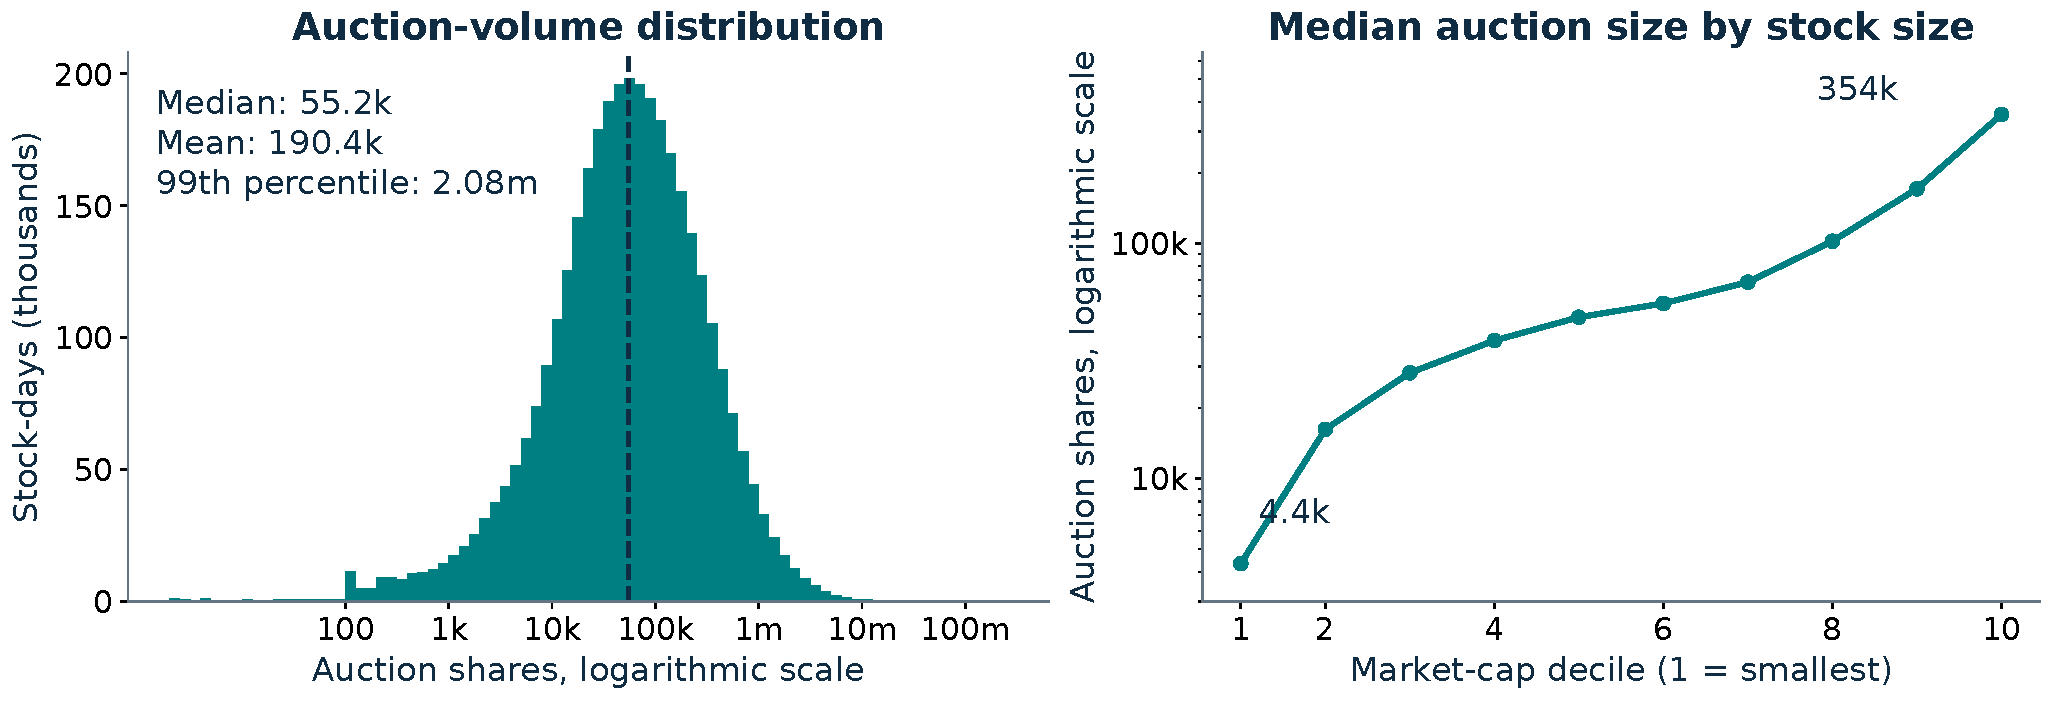
\includegraphics[width=\textwidth,height=4.45cm,keepaspectratio]{assets/descriptive_scale.pdf}
\par\medskip
\raggedright
\textbf{Purpose:} describe the target's distribution and its scale across stocks, motivating proportional and share-scale error measures.
\source{Eligible stock-days, 2015--2025. Size deciles use contemporaneous market capitalization for description. The largest-size decile has about 81 times the median auction volume of the smallest.}
\end{frame}

\begin{frame}{Auction participation: time and calendar comparisons}
\centering
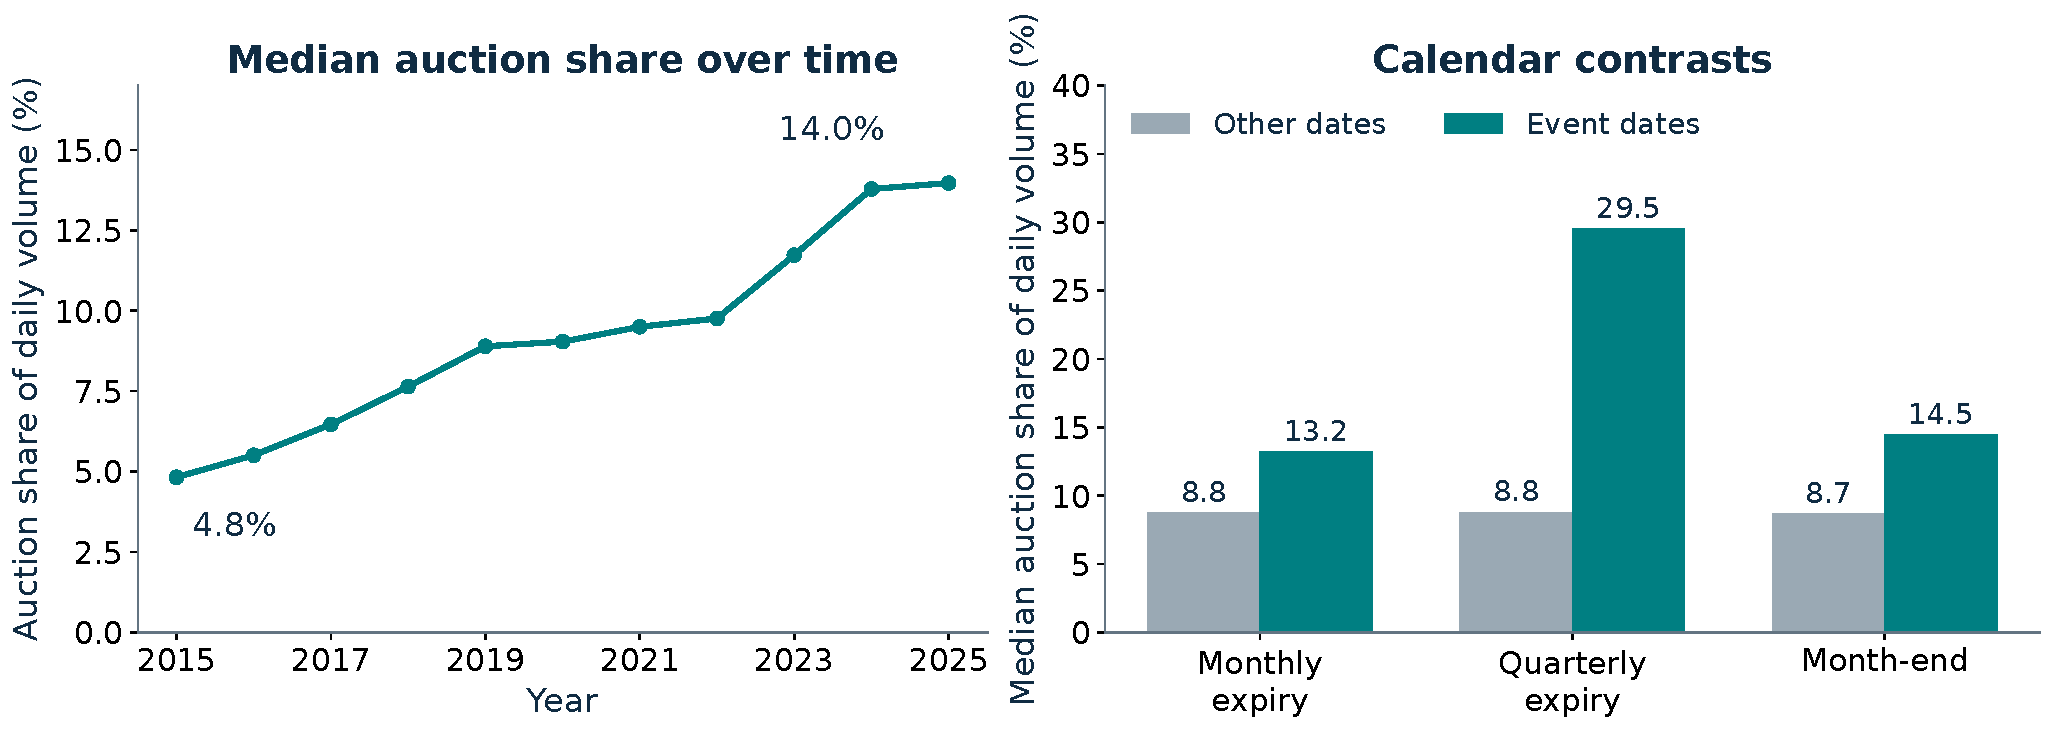
\includegraphics[width=\textwidth,height=4.45cm,keepaspectratio]{assets/descriptive_time_calendar.pdf}
\par\medskip
\raggedright
\textbf{Purpose:} examine participation over time and around calendar events, motivating forward tests and calendar inputs.
\source{Auction share = auction volume / same-day daily volume. Eligible stock-days, 2015--2025. Each event has its own non-event comparison. Groups overlap, and pooled associations do not establish causality.}
\end{frame}

\begin{frame}{Descriptive statistics: summary}
\small
\begin{tabularx}{\textwidth}{@{}L{6.7cm}Y@{}}
\toprule
\textbf{Finding} & \textbf{Implication for the analysis}\\
\midrule
3.50 million eligible labels. Annual observed-target coverage: 93.0\%--99.0\%. & Check coverage and assess accuracy by year.\\[0.8em]
Median auction: 55.2k shares. Mean: 190.4k. 99th percentile: 2.08m. & Report errors in shares and in log space.\\[0.8em]
Largest size-decile median: about 81 times the smallest. & Account for stock scale and compare size groups.\\[0.8em]
Median auction share: 4.8\% in 2015, 14.0\% in 2025, with calendar differences. & Evaluate forward in time and test known calendar flags.\\
\bottomrule
\end{tabularx}
\source{Statistics describe the extracted NYSE sample. Same-day auction share is a descriptive outcome, not an input to the prior-close daily forecast.}
\end{frame}

% Analysis: individual relationships, conditional evidence, target, model, results.
\begin{frame}{Individual covariate relationships with auction volume}
\centering
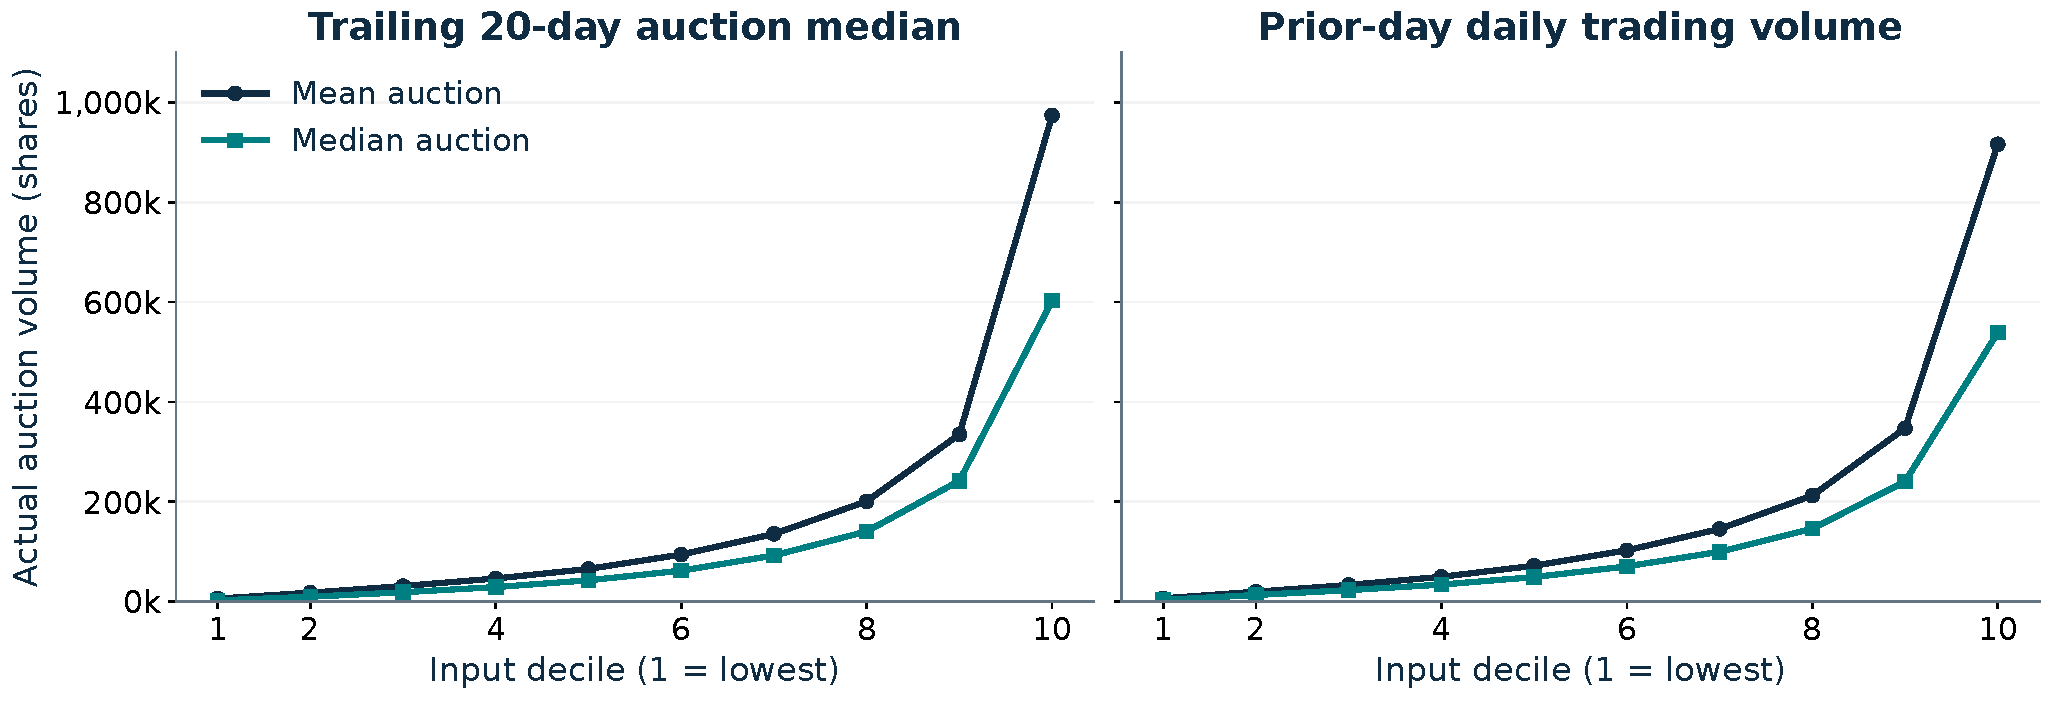
\includegraphics[width=\textwidth,height=4.45cm,keepaspectratio]{assets/analysis_individual_relationships.pdf}
\par\medskip
\raggedright
\textbf{Inference:} recent auction activity and trading volume help describe a stock's normal auction scale.
\source{Individual relationships with auction shares, 2015--2025. Pairwise-complete input deciles keep ties together. These retrospective associations combine stock scale and variation within stocks. They do not measure causal effects or incremental forecast value.}
\end{frame}

\begin{frame}{Stock size and liquidity: individual relationships}
\centering
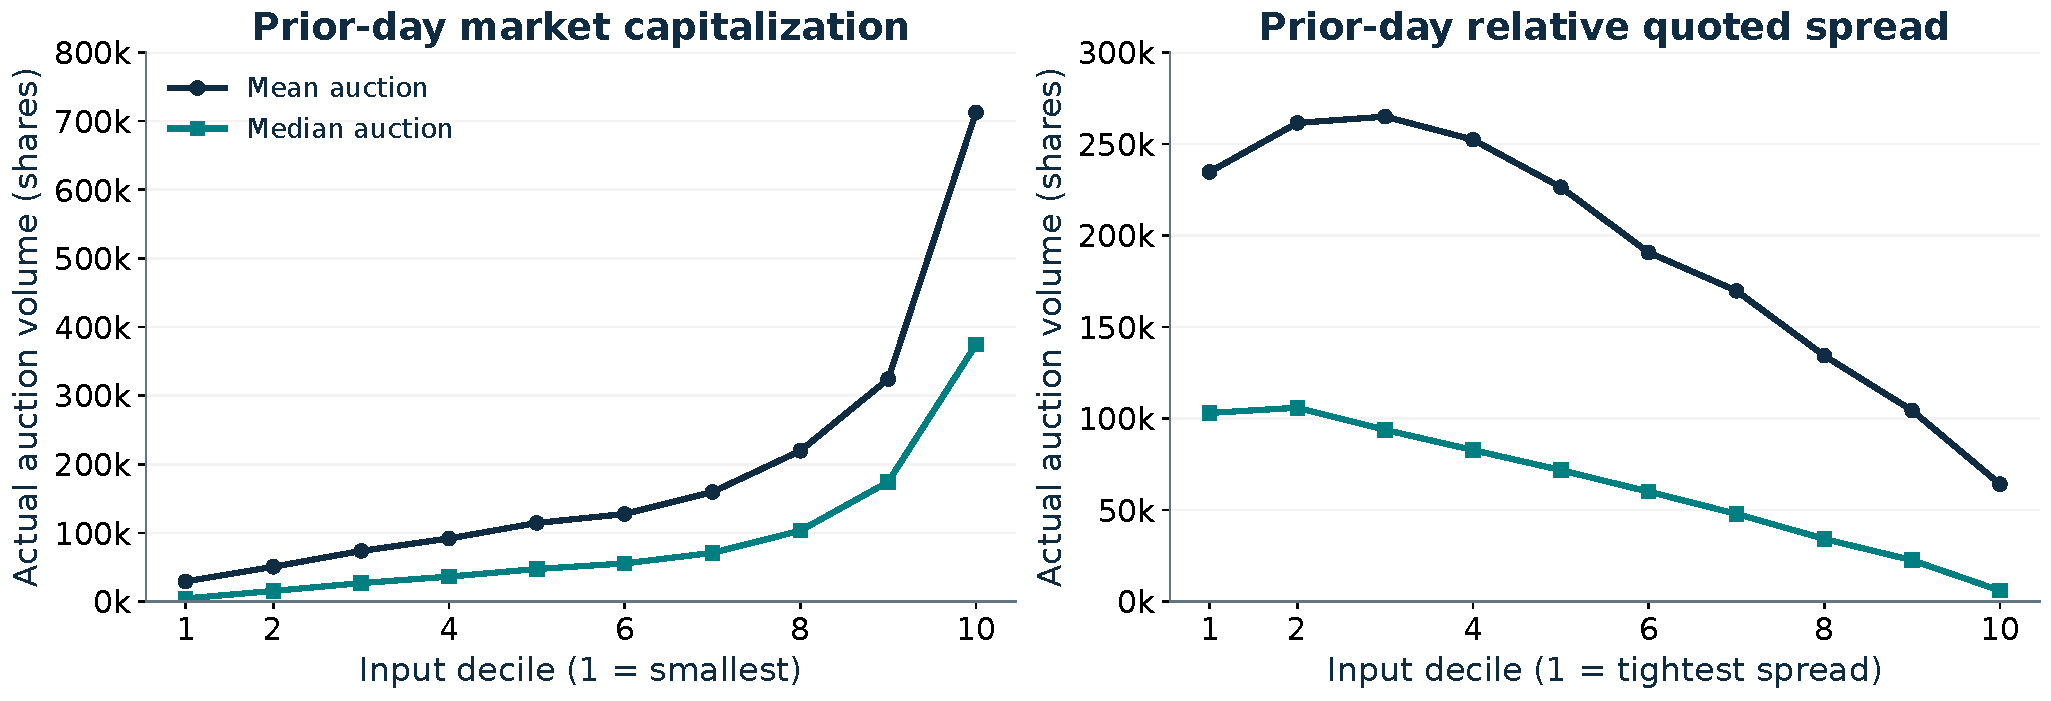
\includegraphics[width=\textwidth,height=4.4cm,keepaspectratio]{assets/covariates_size_spread.pdf}
\par\medskip
\raggedright
\textbf{Inference:} larger stocks and stocks with tighter spreads generally have larger auctions. Much of this pattern reflects differences across stocks.
\source{Auction shares, 2015--2025. Inputs use prior-close values. Pairwise-complete input deciles, with separate vertical ranges. The relative spread uses bid and ask quotes. Pooled relationships do not establish changes within a stock, causal effects, or added forecast value.}
\end{frame}

\begin{frame}{Stock returns and auction volume}
\centering
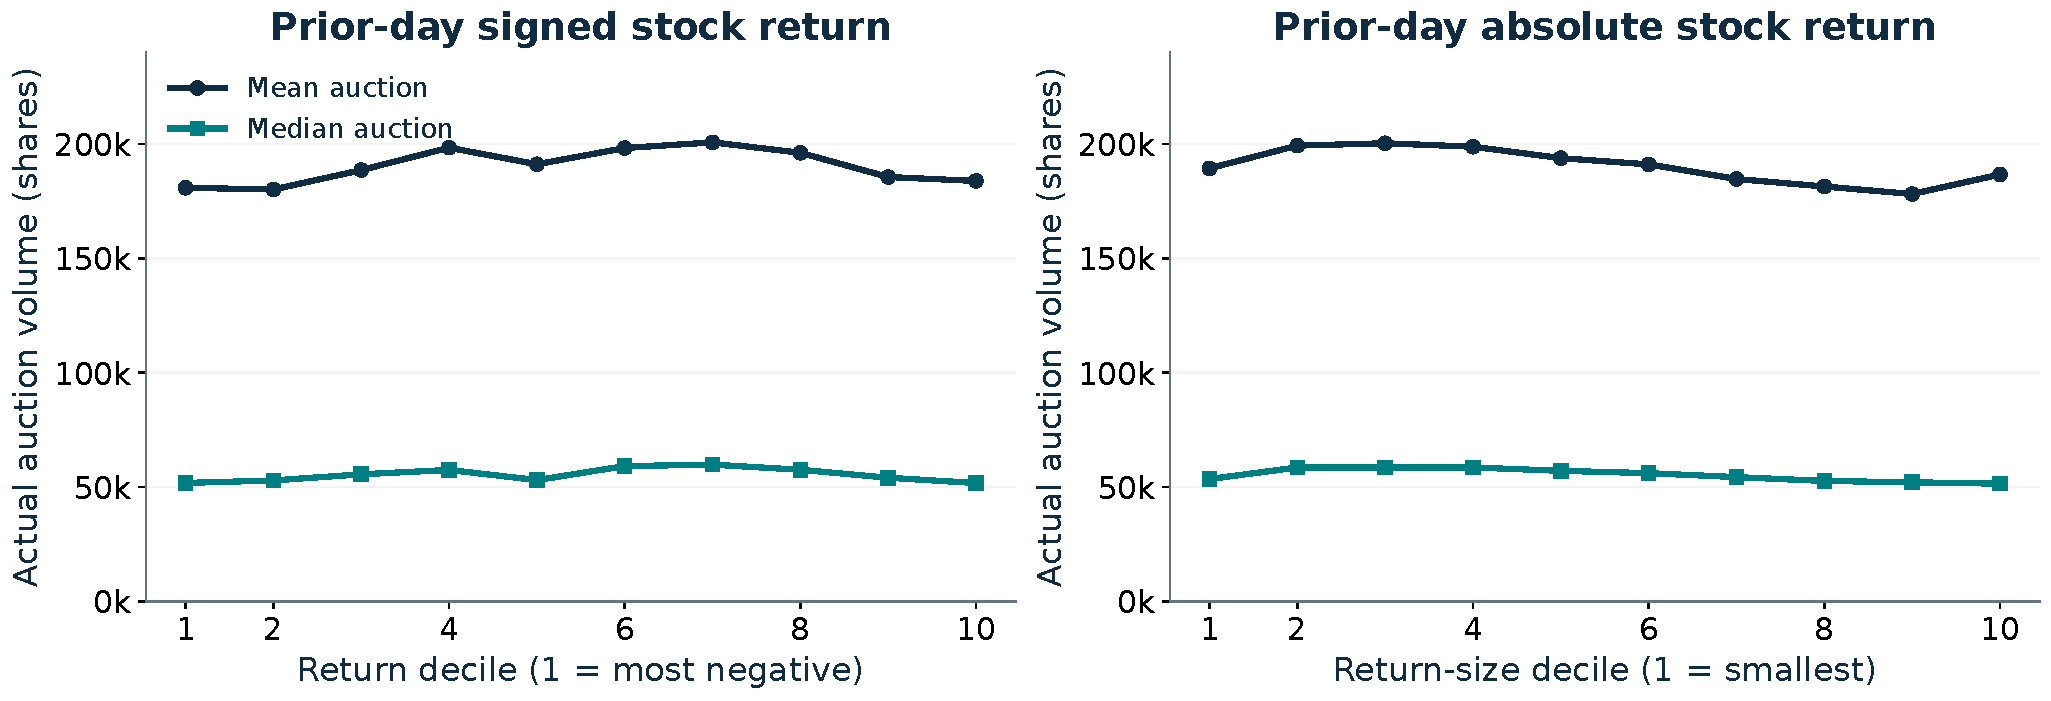
\includegraphics[width=\textwidth,height=4.4cm,keepaspectratio]{assets/covariates_returns.pdf}
\par\medskip
\raggedright
\textbf{Inference:} neither signed nor absolute prior-day return shows a strong monotonic relationship with auction size in these pooled curves.
\source{Auction shares, 2015--2025. Signed-return groups run from most negative to most positive. Absolute-return groups run from smallest to largest moves. Inputs are lagged. Pairwise-complete pooled associations do not rule out nonlinear or conditional relationships.}
\end{frame}

\begin{frame}{Market and sector activity: individual relationships}
\centering
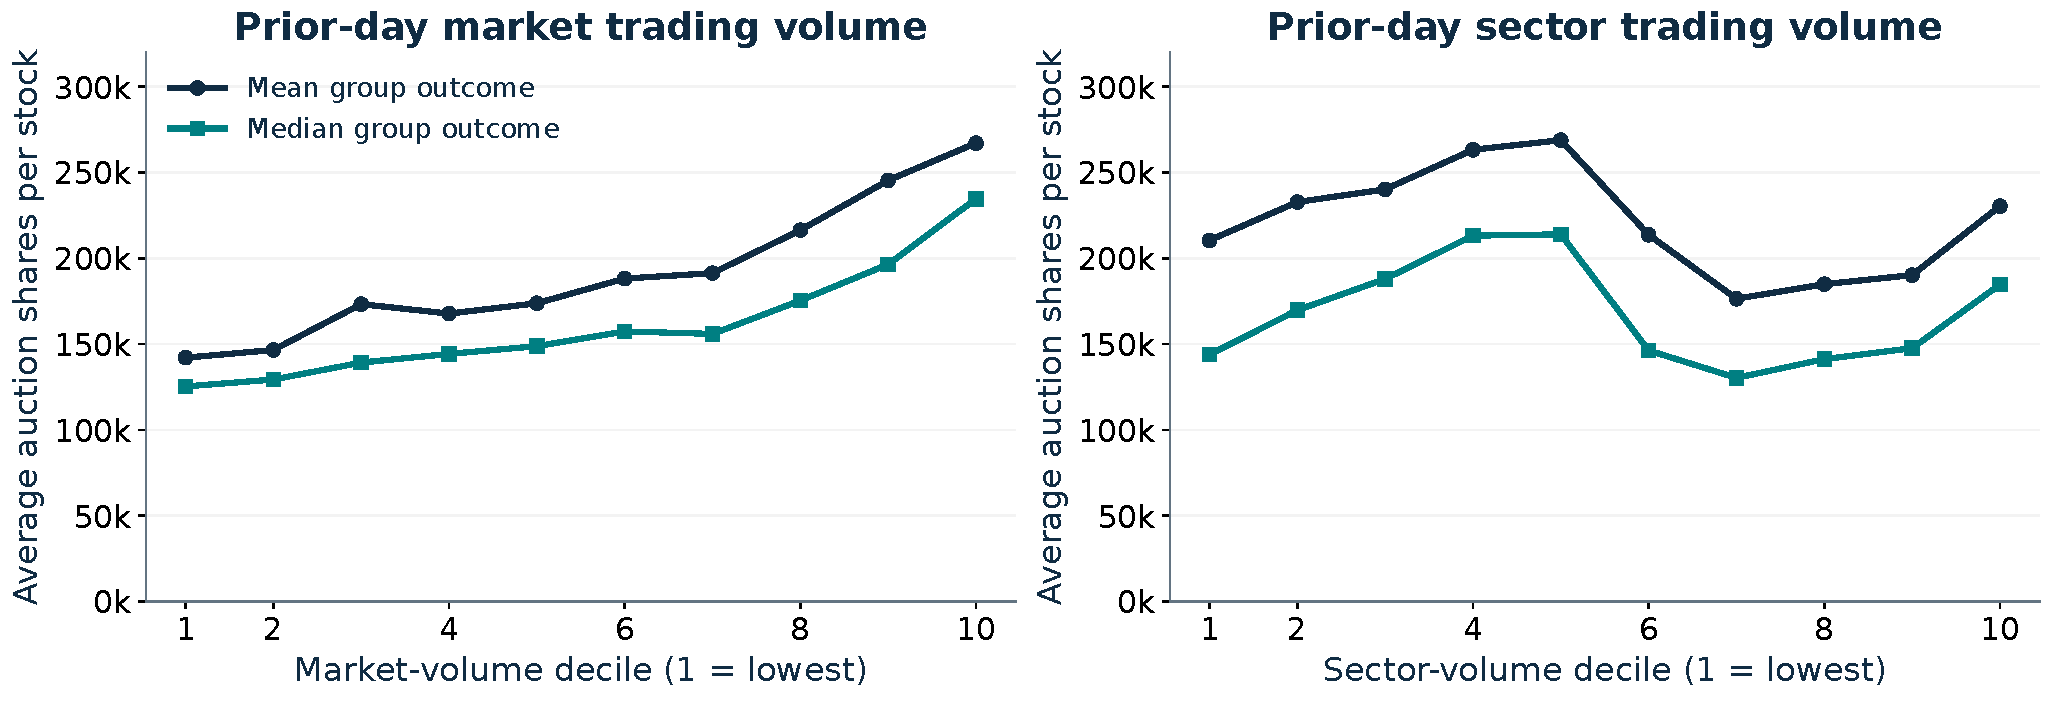
\includegraphics[width=\textwidth,height=4.4cm,keepaspectratio]{assets/covariates_market_sector.pdf}
\par\medskip
\raggedright
\textbf{Inference:} higher market activity accompanies larger average auctions. The pooled sector relationship varies across volume groups.
\source{Prior-day inputs, 2015--2025. Left outcome: daily mean auction shares per eligible stock. Right outcome: sector-day mean. Lines summarize the mean and median of those group outcomes within input deciles. Dates or sector-days receive equal weight. Composition, trends, and sector differences remain uncontrolled.}
\end{frame}

\begin{frame}{Feature-family removal tests}
\centering
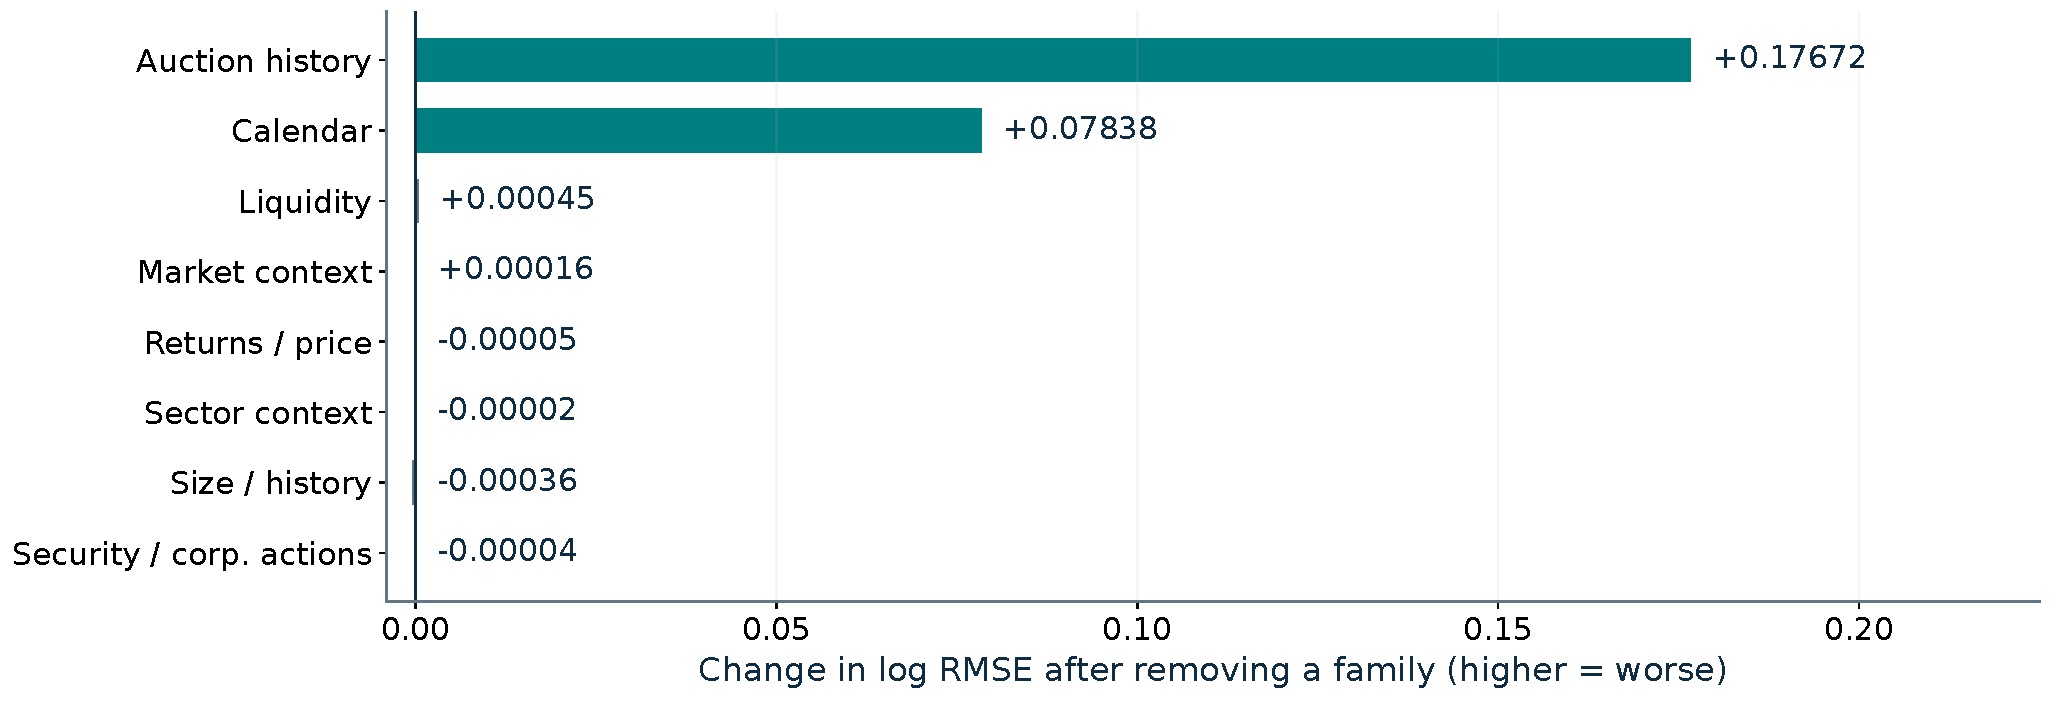
\includegraphics[width=\textwidth,height=4.15cm,keepaspectratio]{assets/analysis_family_ablation.pdf}
\par\medskip
\raggedright
\textbf{Inference:} auction history and calendar information contribute most. Liquidity's additional gain is small and depends on the error metric.
\source{Controlled ridge audit, mean annual 2022--2024 log RMSE. Remove one family at a time from the full model with other settings held fixed. This earlier audit uses direct log levels and an expanding training history. Small changes do not prove that individual inputs are unnecessary.}
\end{frame}

\begin{frame}{Target formulation: deviation from the 20-day median}
\lead{Learn a correction to each stock's recent typical auction}
Let $B_{i,t}$ be the trailing 20-day auction median, using only observations before $t$.
\[
 r_{i,t}=\log(1+A_{i,t})-\log(1+B_{i,t})
\]
\[
 \widehat A_{i,t}=\max\!\left\{0,\ \exp\!\left[\log(1+B_{i,t})+\widehat r_{i,t}\right]-1\right\}
\]
\medskip
\begin{tabularx}{\textwidth}{@{}Y r@{}}
\toprule
\textbf{Controlled target comparison} & \textbf{Development log RMSE}\\
\midrule
Direct log level & 0.49609\\[0.3em]
Deviation from the median in log space & \textbf{0.48710}\\
\bottomrule
\end{tabularx}
\source{Same five-year rolling history, 99 source features, and uniform weights. Mean annual 2022--2024 log RMSE, lower is better. Missing baselines use a historical training-median fallback. The business target remains auction shares. Forecast safeguards also use historical training bounds.}
\end{frame}

\begin{frame}{Ridge benchmark: specification comparison}
\lead{One modeling approach explored so far}
\small
\begin{tabularx}{\textwidth}{@{}Y r r@{}}
\toprule
\textbf{Ridge specification} & \textbf{Inputs} & \textbf{Development log RMSE}\\
\midrule
Full feature set, more weight on recent days & 99 & 0.48677\\[0.5em]
\textbf{Auction / calendar / liquidity, equal row weights} & \textbf{58} & \textbf{0.48764}\\[0.5em]
Auction / calendar, equal row weights & 42 & 0.49059\\
\bottomrule
\end{tabularx}
\medskip
\normalsize
\begin{points}
\item \textbf{Within these ridge trials:} prefer fewer inputs within 0.002 of the best mean annual development log RMSE.
\item \textbf{Reference specification:} global ridge, five-year rolling history, equal training-row weights. 19 auction-history + 23 calendar + 16 liquidity inputs.
\end{points}
\source{Training weights control each stock-day's contribution to fitting error. Equal weights treat every row equally. Recent-data weights decay with age, with a two-year half-life. Development: 2022--2024. Input counts precede encoding and missingness indicators.}
\end{frame}

\begin{frame}{Annual forecast errors: ridge versus recent median}
\small
\textbf{Recent-median rule:} the prediction is simply the stock's trailing 20-day auction median.\par
\medskip
\centering
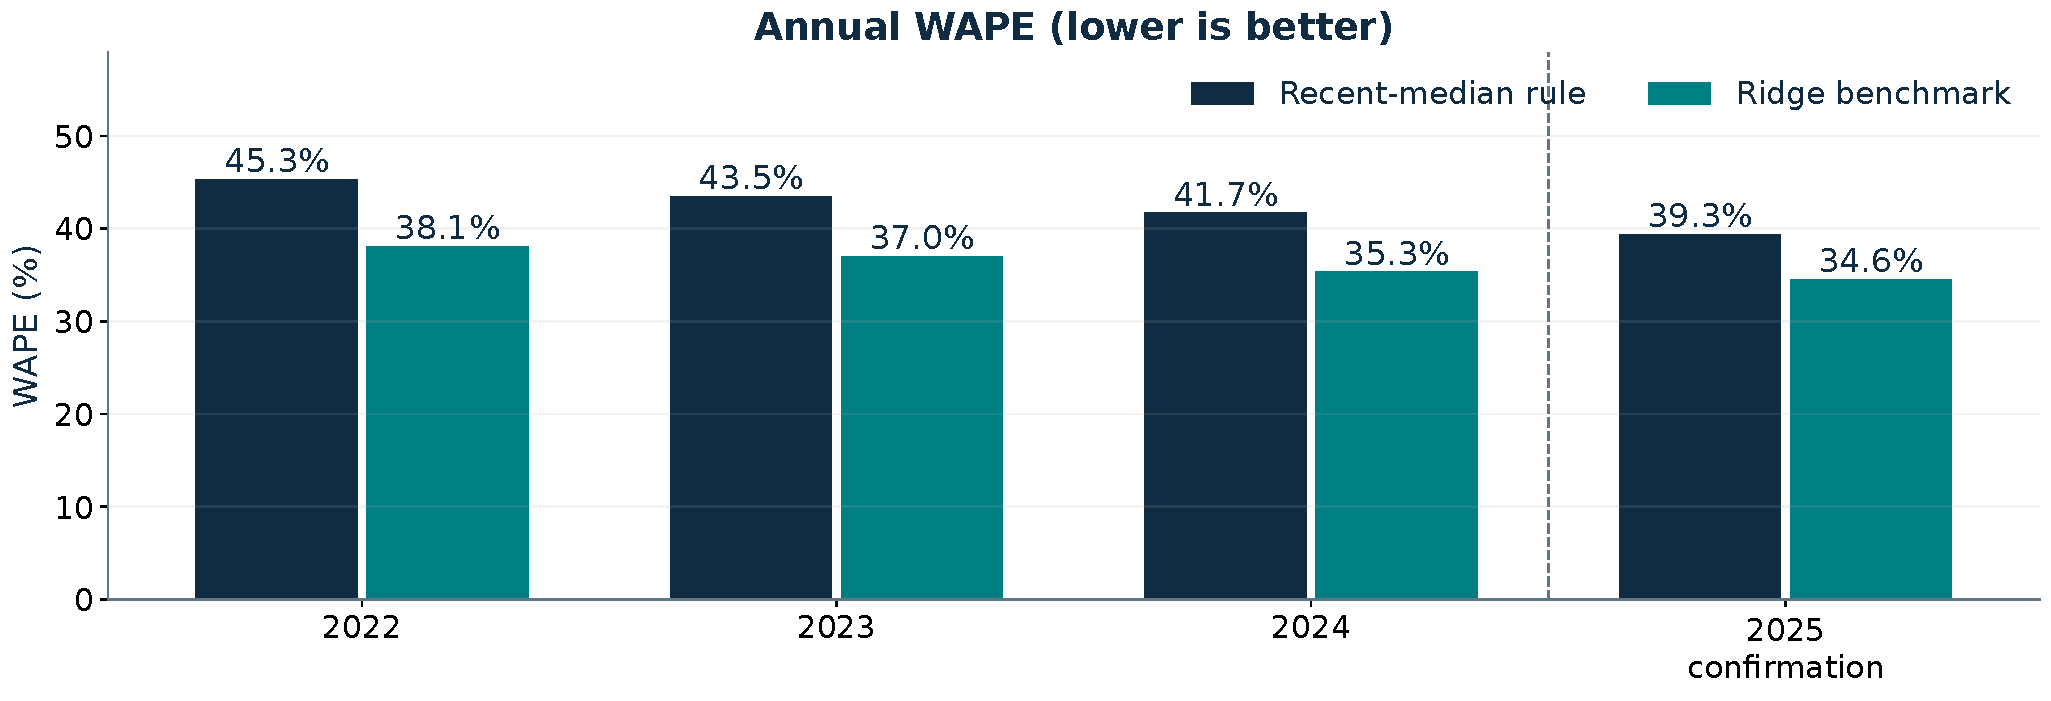
\includegraphics[width=\textwidth,height=3.55cm,keepaspectratio]{assets/analysis_forward_performance.pdf}
\par\medskip
\raggedright
\small
\textbf{Mean annual WAPE, 2022--2024:} 43.47\% median rule, 36.80\% ridge.\par\smallskip
\textbf{Meaning:} 36.8\% WAPE corresponds to 36.8 shares of total absolute error per 100 actual shares. Substantial error remains.
\source{The median uses only earlier observations, with a training-median fallback if unavailable. WAPE = total absolute share error / total actual shares. The headline averages annual WAPEs on common rows. The 2025 confirmation year had already been inspected during research.}
\end{frame}

\begin{frame}{Actual versus predicted volume: 20-day rolling medians}
\centering
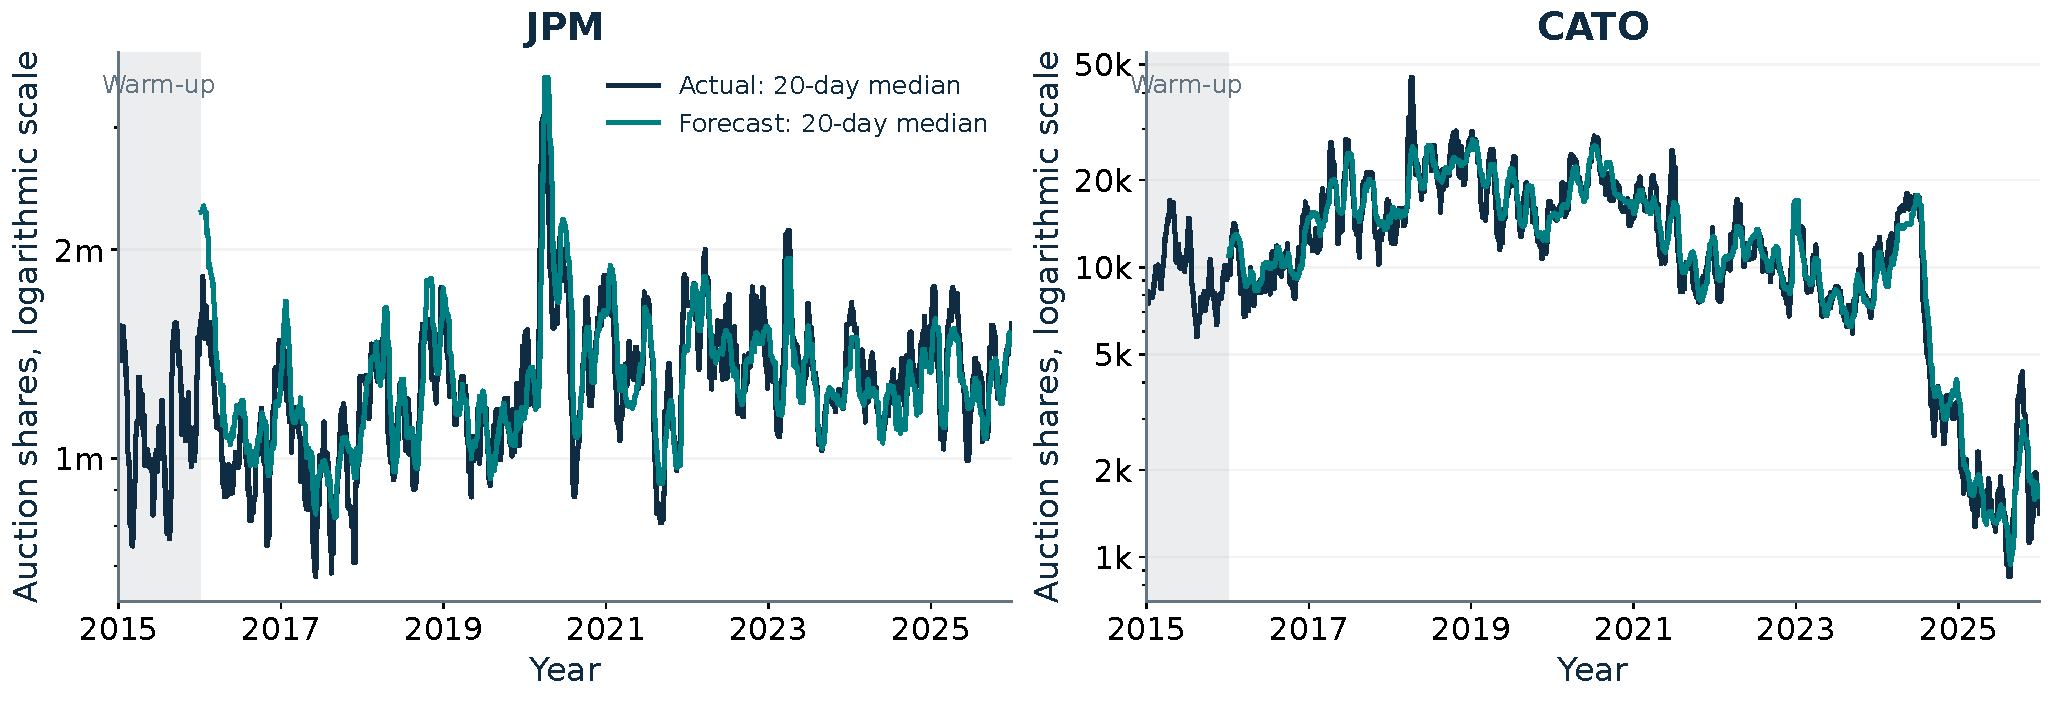
\includegraphics[width=\textwidth,height=4.4cm,keepaspectratio]{assets/backtest_rolling_medians.pdf}
\par\medskip
\raggedright
\textbf{Inference:} the smoothed forecasts follow changes in typical activity. Daily errors require a separate view.
\source{Trailing 20-trading-observation medians of actual and predicted shares, minimum five non-missing values per series. Logarithmic axes with separate ranges. 2015 is actuals-only warm-up. Forecasts begin in 2016 and use earlier fitting data. The model specification was selected retrospectively.}
\end{frame}

\begin{frame}{Daily actual versus predicted auction volume}
\centering
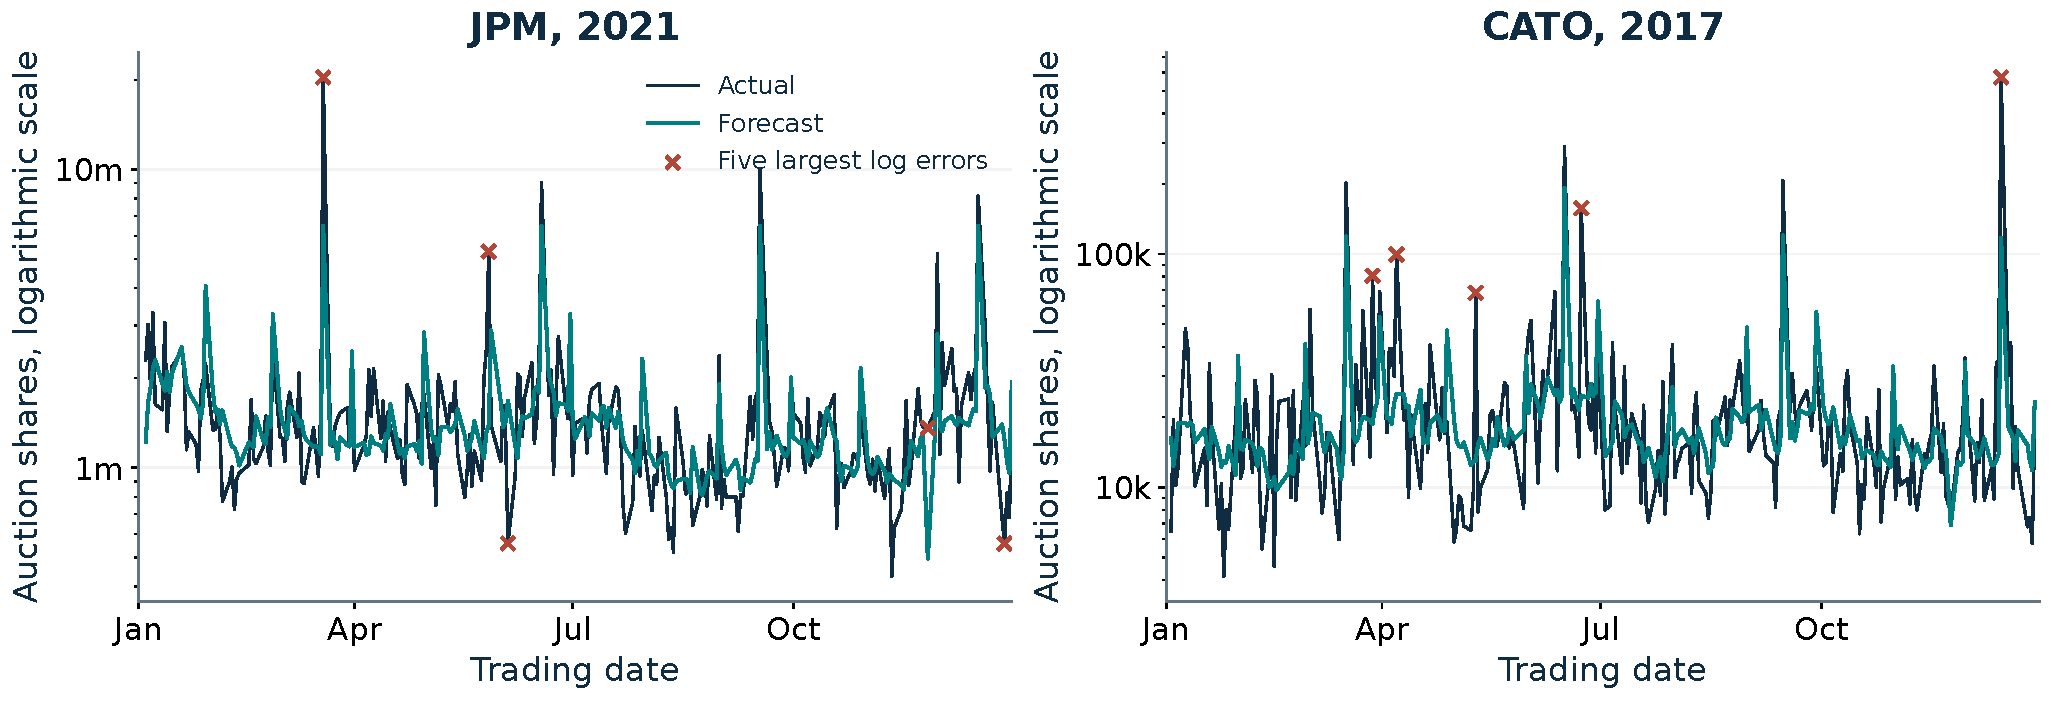
\includegraphics[width=\textwidth,height=3.55cm,keepaspectratio]{assets/backtest_daily_examples.pdf}
\par\smallskip
\raggedright
\small
\begin{tabularx}{\textwidth}{@{}Y r r@{}}
\toprule
\textbf{Example} & \textbf{Median-rule WAPE} & \textbf{Ridge WAPE}\\
\midrule
JPM, 2021 & 37.9\% & 30.8\%\\
CATO, 2017 & 56.6\% & 46.4\%\\
\bottomrule
\end{tabularx}
\par\smallskip
\textbf{Inference:} ridge improves on the median rule in these examples, but absolute errors remain substantial.
\source{Unsmoothed daily actuals and walk-forward forecasts. Each example year is nearest its stock's median annual log RMSE over 2016--2025. Years and axis ranges differ. The model specification was selected retrospectively. Crosses mark the five largest absolute log errors in each example.}
\end{frame}

\begin{frame}{Remaining challenges}
\lead{Overall gains leave important gaps across auctions and stocks}
\begin{points}
\item \textbf{Large auctions and sharp spikes}\par
Tail forecasts remain too low, and daily case studies reveal missed spikes. Their economic causes still need investigation.
\item \textbf{Small stocks and limited history}\par
Errors are higher in these groups. Uneven coverage and limited auction history complicate reliable forecasts.
\item \textbf{Information arriving during the day}\par
The daily forecast uses the previous close. It cannot respond to announcement outcomes or trading activity observed later.
\end{points}
\source{Challenges follow the forward evaluations and stock-level diagnostics. Group differences and missed spikes do not establish their causes.}
\end{frame}

\begin{frame}{Roadmap and next steps}
\small
\renewcommand{\arraystretch}{1.1}
\begin{tabularx}{\textwidth}{@{}L{3.2cm}Y@{}}
\toprule
\textbf{Sequence} & \textbf{Planned analysis}\\
\midrule
\textbf{1. Diagnose errors and refine history} & Review large misses, coverage, and limited-history fallbacks. Test adaptation to changing stock activity.\\[0.6em]
\textbf{2. Test nonlinear models} & Compare ridge with nonlinear models, such as boosted trees, to test thresholds and feature interactions.\\[0.6em]
\textbf{3. Test daily context} & Evaluate lagged VIX/rates and scheduled CPI/NFP indicators beyond the existing calendar inputs.\\[0.6em]
\textbf{4. Develop intraday updates} & Update the daily forecast using trading activity at the prepared checkpoints.\\
\bottomrule
\end{tabularx}
\par\vspace{0.35cm}
\normalsize
\textbf{Evaluation:} compare against a fixed ridge reference on chronological folds and additional periods unused in development.
\source{Planned extensions, with gains still to be tested. Compare model classes on the same information set before adding new inputs. Daily features must be available at the previous close or known in advance. CPI = Consumer Price Index. NFP = nonfarm payrolls.}
\end{frame}

\appendix
\setbeamertemplate{footline}{}
\begin{frame}[noframenumbering]{Ridge diagnostic: training and evaluation stages}
\lead{One ridge specification across three evaluation stages}
\centering
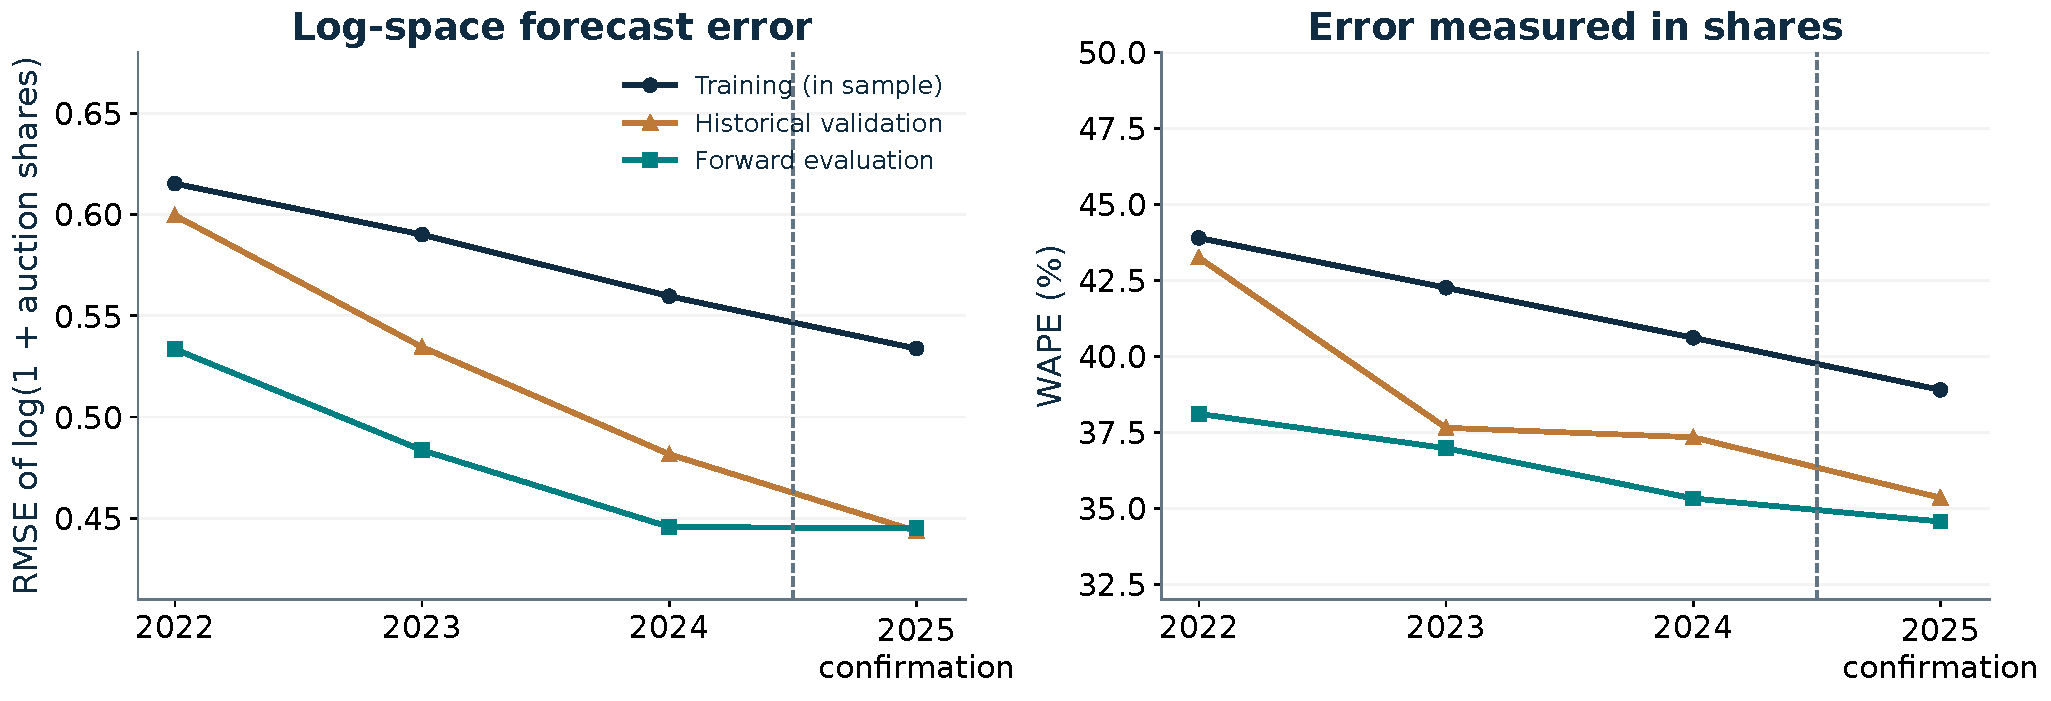
\includegraphics[width=\textwidth,height=3.65cm,keepaspectratio]{assets/backtest_train_validation_test.pdf}
\par\medskip
\raggedright
{\small \textbf{Purpose:} examine errors during fitting, tuning, and later-year forecasting. This graph does not compare ridge with the median rule.\par}
\source{Training: 350k sampled rows per fold. Historical validation: 120k rows from an earlier year. Forward evaluation: all eligible forecast-year rows. Periods, samples, and fitted stages differ, so lower forward error alone cannot rule out overfitting. The 2025 confirmation year had already been inspected during research.}
\end{frame}

\begin{frame}[noframenumbering]{References: background literature}
\small
\textbf{[L1]} Bogousslavsky, V., and Muravyev, D. (2023). Who trades at the close? Implications for price discovery and liquidity. \emph{Journal of Financial Markets}, 66, 100852.\par
\href{https://doi.org/10.1016/j.finmar.2023.100852}{doi:10.1016/j.finmar.2023.100852}\par\bigskip
\textbf{[L2]} Kandel, E., Rindi, B., and Bosetti, L. (2012). The effect of a closing call auction on market quality and trading strategies. \emph{Journal of Financial Intermediation}, 21(1), 23--49.\par
\href{https://iris.unibocconi.it/handle/11565/2646191}{Bocconi research record and abstract}\par\bigskip
\textbf{[L3]} Bia{\l}kowski, J., Darolles, S., and Le Fol, G. (2008). Improving VWAP strategies: A dynamic volume approach. \emph{Journal of Banking \& Finance}, 32(9), 1709--1722.\par
\href{https://doi.org/10.1016/j.jbankfin.2007.09.023}{doi:10.1016/j.jbankfin.2007.09.023}
\end{frame}


\end{document}
